% Created by tikzDevice version 0.12.3.1 on 2021-12-16 11:00:05
% !TEX encoding = UTF-8 Unicode
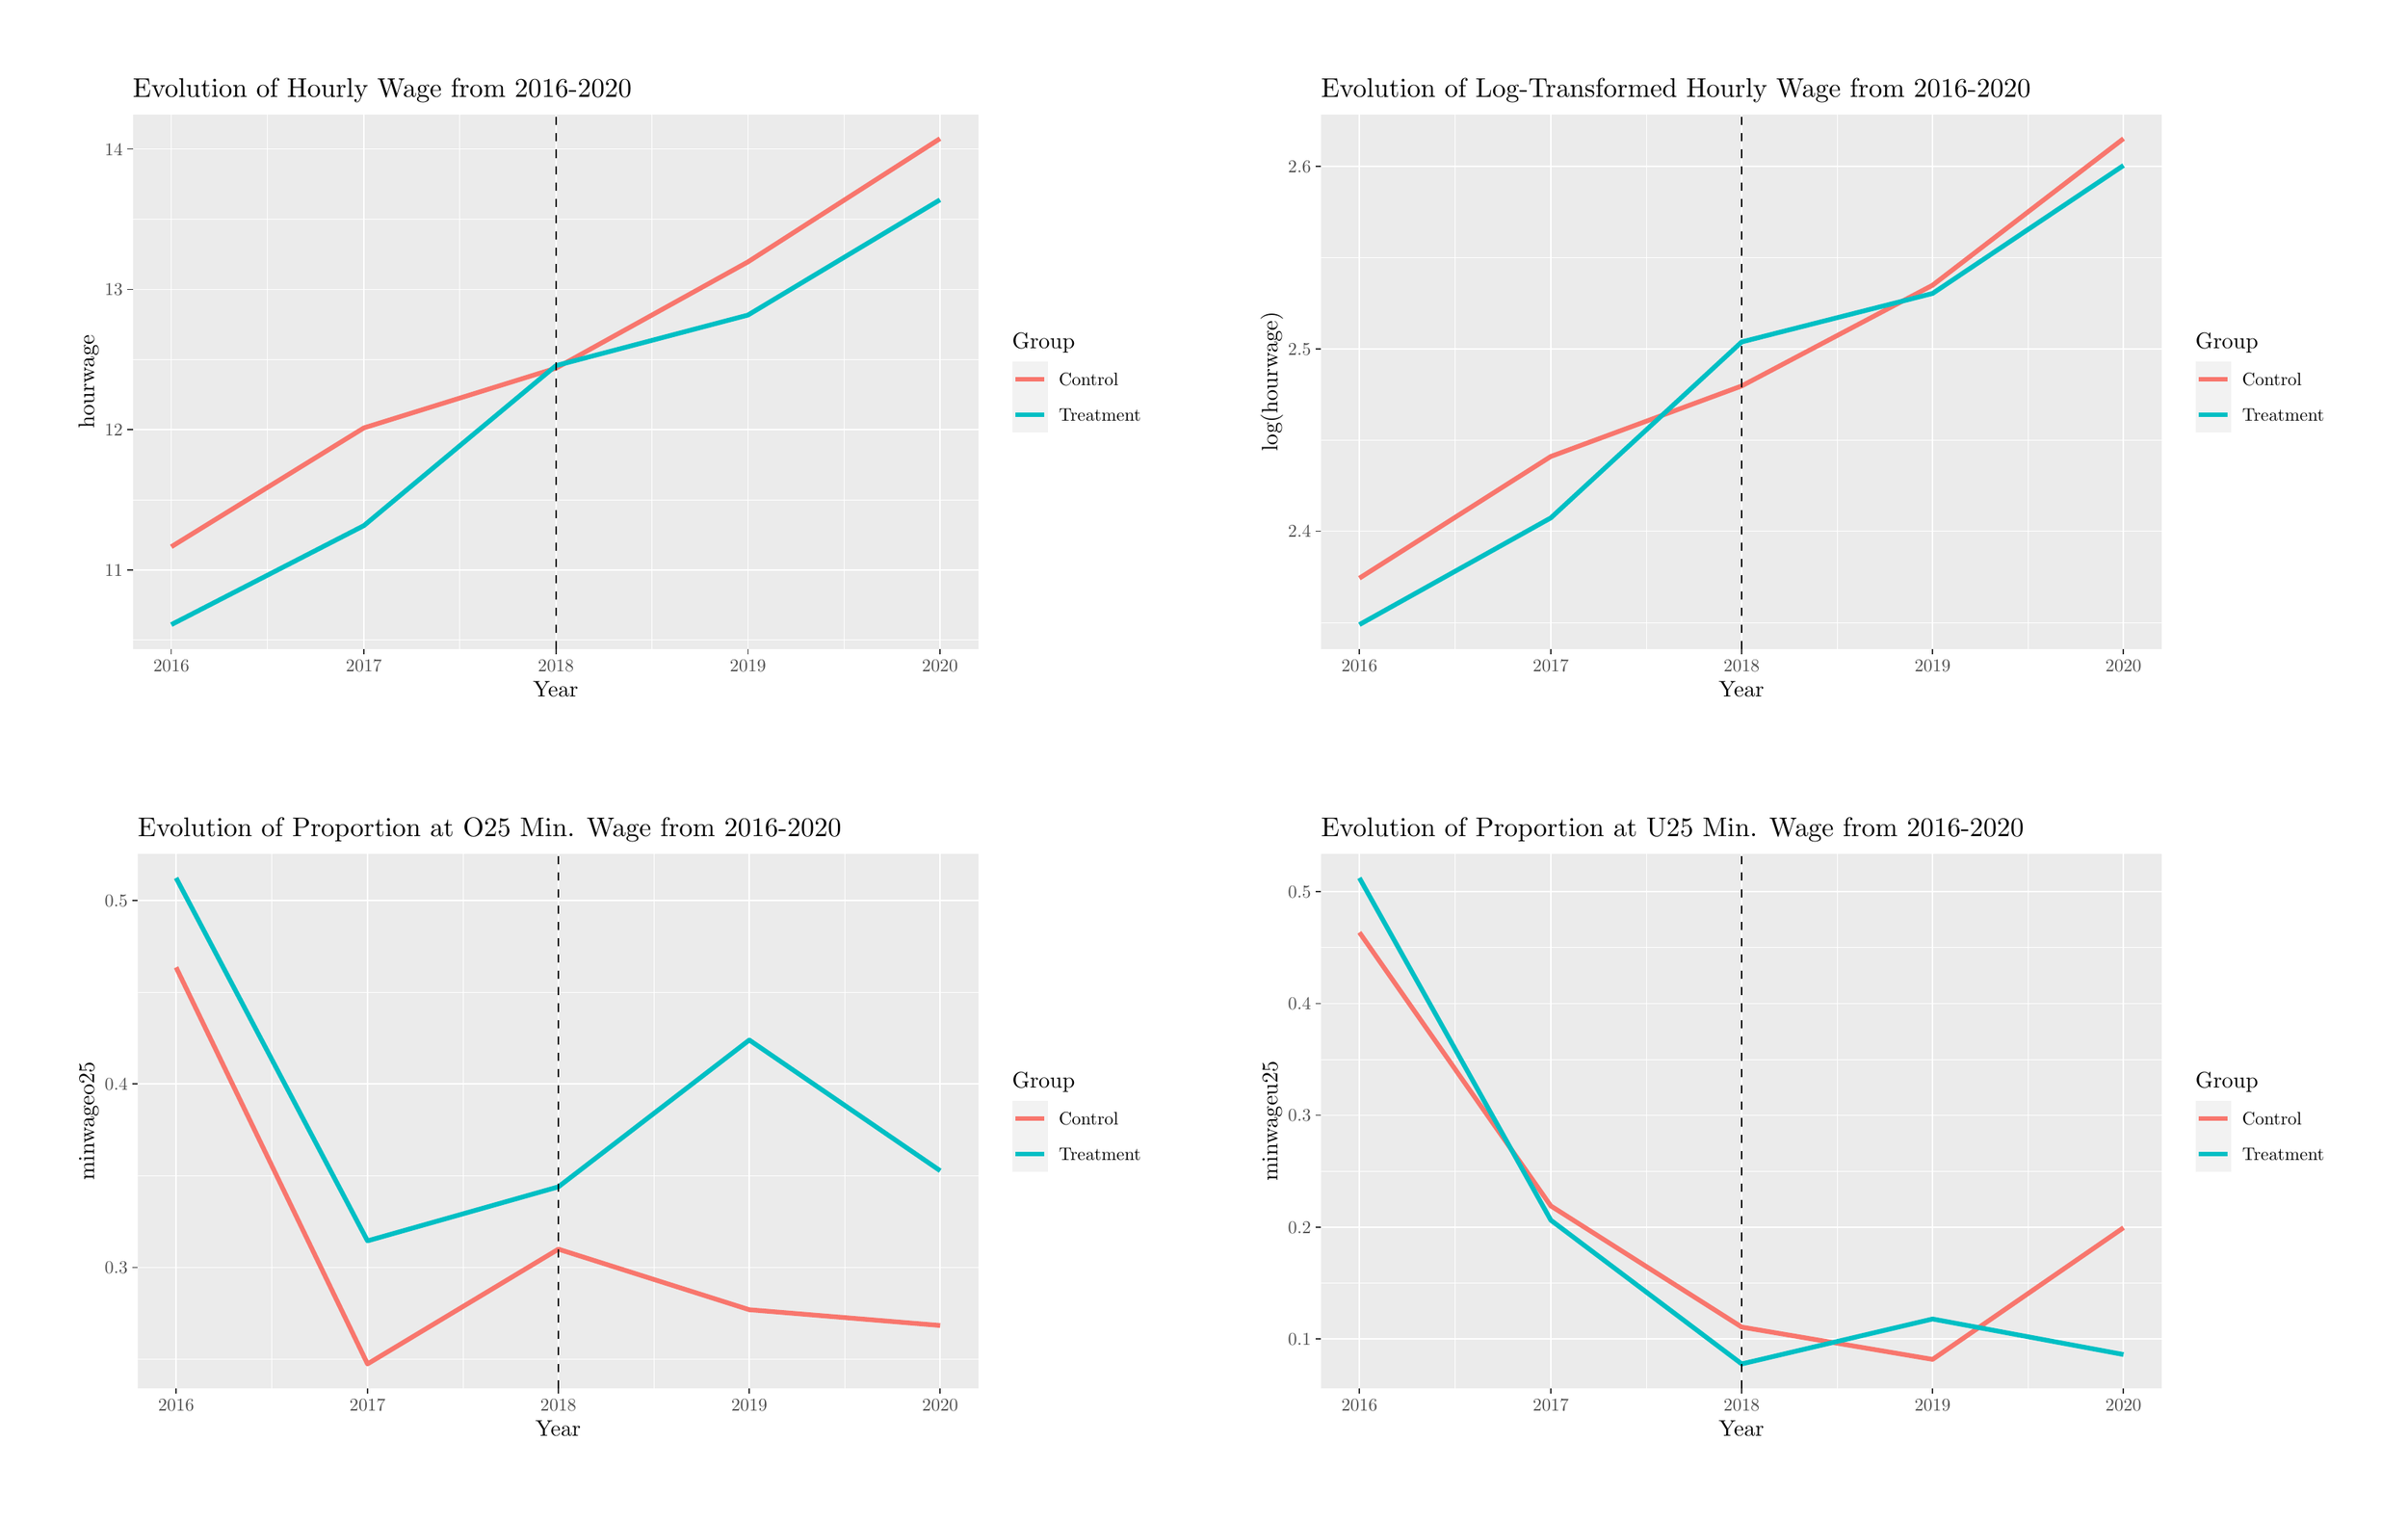
\begin{tikzpicture}[x=1pt,y=1pt]
\definecolor{fillColor}{RGB}{255,255,255}
\path[use as bounding box,fill=fillColor,fill opacity=0.00] (0,0) rectangle (1156.32,722.70);
\begin{scope}
\path[clip] (  0.00,361.35) rectangle (578.16,722.70);
\definecolor{drawColor}{RGB}{255,255,255}
\definecolor{fillColor}{RGB}{255,255,255}

\path[draw=drawColor,line width= 0.6pt,line join=round,line cap=round,fill=fillColor] (  0.00,361.35) rectangle (578.16,722.70);
\end{scope}
\begin{scope}
\path[clip] ( 54.93,415.52) rectangle (468.05,676.81);
\definecolor{fillColor}{gray}{0.92}

\path[fill=fillColor] ( 54.93,415.52) rectangle (468.05,676.81);
\definecolor{drawColor}{RGB}{255,255,255}

\path[draw=drawColor,line width= 0.3pt,line join=round] ( 54.93,419.81) --
	(468.05,419.81);

\path[draw=drawColor,line width= 0.3pt,line join=round] ( 54.93,488.39) --
	(468.05,488.39);

\path[draw=drawColor,line width= 0.3pt,line join=round] ( 54.93,556.97) --
	(468.05,556.97);

\path[draw=drawColor,line width= 0.3pt,line join=round] ( 54.93,625.55) --
	(468.05,625.55);

\path[draw=drawColor,line width= 0.3pt,line join=round] (120.75,415.52) --
	(120.75,676.81);

\path[draw=drawColor,line width= 0.3pt,line join=round] (214.71,415.52) --
	(214.71,676.81);

\path[draw=drawColor,line width= 0.3pt,line join=round] (308.53,415.52) --
	(308.53,676.81);

\path[draw=drawColor,line width= 0.3pt,line join=round] (402.36,415.52) --
	(402.36,676.81);

\path[draw=drawColor,line width= 0.6pt,line join=round] ( 54.93,454.10) --
	(468.05,454.10);

\path[draw=drawColor,line width= 0.6pt,line join=round] ( 54.93,522.68) --
	(468.05,522.68);

\path[draw=drawColor,line width= 0.6pt,line join=round] ( 54.93,591.26) --
	(468.05,591.26);

\path[draw=drawColor,line width= 0.6pt,line join=round] ( 54.93,659.83) --
	(468.05,659.83);

\path[draw=drawColor,line width= 0.6pt,line join=round] ( 73.71,415.52) --
	( 73.71,676.81);

\path[draw=drawColor,line width= 0.6pt,line join=round] (167.79,415.52) --
	(167.79,676.81);

\path[draw=drawColor,line width= 0.6pt,line join=round] (261.62,415.52) --
	(261.62,676.81);

\path[draw=drawColor,line width= 0.6pt,line join=round] (355.45,415.52) --
	(355.45,676.81);

\path[draw=drawColor,line width= 0.6pt,line join=round] (449.27,415.52) --
	(449.27,676.81);
\definecolor{drawColor}{RGB}{248,118,109}

\path[draw=drawColor,line width= 2.3pt,line join=round] ( 73.71,465.46) --
	(167.79,523.54) --
	(261.62,552.72) --
	(355.45,604.68) --
	(449.27,664.93);
\definecolor{drawColor}{RGB}{0,191,196}

\path[draw=drawColor,line width= 2.3pt,line join=round] ( 73.71,427.39) --
	(167.79,475.77) --
	(261.62,553.97) --
	(355.45,578.69) --
	(449.27,635.03);
\definecolor{drawColor}{RGB}{0,0,0}

\path[draw=drawColor,line width= 0.6pt,dash pattern=on 4pt off 4pt ,line join=round] (261.62,415.52) -- (261.62,676.81);
\end{scope}
\begin{scope}
\path[clip] (  0.00,  0.00) rectangle (1156.32,722.70);
\definecolor{drawColor}{gray}{0.30}

\node[text=drawColor,anchor=base east,inner sep=0pt, outer sep=0pt, scale=  0.88] at ( 49.98,451.07) {11};

\node[text=drawColor,anchor=base east,inner sep=0pt, outer sep=0pt, scale=  0.88] at ( 49.98,519.65) {12};

\node[text=drawColor,anchor=base east,inner sep=0pt, outer sep=0pt, scale=  0.88] at ( 49.98,588.23) {13};

\node[text=drawColor,anchor=base east,inner sep=0pt, outer sep=0pt, scale=  0.88] at ( 49.98,656.80) {14};
\end{scope}
\begin{scope}
\path[clip] (  0.00,  0.00) rectangle (1156.32,722.70);
\definecolor{drawColor}{gray}{0.20}

\path[draw=drawColor,line width= 0.6pt,line join=round] ( 52.18,454.10) --
	( 54.93,454.10);

\path[draw=drawColor,line width= 0.6pt,line join=round] ( 52.18,522.68) --
	( 54.93,522.68);

\path[draw=drawColor,line width= 0.6pt,line join=round] ( 52.18,591.26) --
	( 54.93,591.26);

\path[draw=drawColor,line width= 0.6pt,line join=round] ( 52.18,659.83) --
	( 54.93,659.83);
\end{scope}
\begin{scope}
\path[clip] (  0.00,  0.00) rectangle (1156.32,722.70);
\definecolor{drawColor}{gray}{0.20}

\path[draw=drawColor,line width= 0.6pt,line join=round] ( 73.71,412.77) --
	( 73.71,415.52);

\path[draw=drawColor,line width= 0.6pt,line join=round] (167.79,412.77) --
	(167.79,415.52);

\path[draw=drawColor,line width= 0.6pt,line join=round] (261.62,412.77) --
	(261.62,415.52);

\path[draw=drawColor,line width= 0.6pt,line join=round] (355.45,412.77) --
	(355.45,415.52);

\path[draw=drawColor,line width= 0.6pt,line join=round] (449.27,412.77) --
	(449.27,415.52);
\end{scope}
\begin{scope}
\path[clip] (  0.00,  0.00) rectangle (1156.32,722.70);
\definecolor{drawColor}{gray}{0.30}

\node[text=drawColor,anchor=base,inner sep=0pt, outer sep=0pt, scale=  0.88] at ( 73.71,404.51) {2016};

\node[text=drawColor,anchor=base,inner sep=0pt, outer sep=0pt, scale=  0.88] at (167.79,404.51) {2017};

\node[text=drawColor,anchor=base,inner sep=0pt, outer sep=0pt, scale=  0.88] at (261.62,404.51) {2018};

\node[text=drawColor,anchor=base,inner sep=0pt, outer sep=0pt, scale=  0.88] at (355.45,404.51) {2019};

\node[text=drawColor,anchor=base,inner sep=0pt, outer sep=0pt, scale=  0.88] at (449.27,404.51) {2020};
\end{scope}
\begin{scope}
\path[clip] (  0.00,  0.00) rectangle (1156.32,722.70);
\definecolor{drawColor}{RGB}{0,0,0}

\node[text=drawColor,anchor=base,inner sep=0pt, outer sep=0pt, scale=  1.10] at (261.49,392.21) {Year};
\end{scope}
\begin{scope}
\path[clip] (  0.00,  0.00) rectangle (1156.32,722.70);
\definecolor{drawColor}{RGB}{0,0,0}

\node[text=drawColor,rotate= 90.00,anchor=base,inner sep=0pt, outer sep=0pt, scale=  1.10] at ( 36.03,546.16) {hourwage};
\end{scope}
\begin{scope}
\path[clip] (  0.00,  0.00) rectangle (1156.32,722.70);
\definecolor{fillColor}{RGB}{255,255,255}

\path[fill=fillColor] (479.05,515.71) rectangle (549.71,576.62);
\end{scope}
\begin{scope}
\path[clip] (  0.00,  0.00) rectangle (1156.32,722.70);
\definecolor{drawColor}{RGB}{0,0,0}

\node[text=drawColor,anchor=base west,inner sep=0pt, outer sep=0pt, scale=  1.10] at (484.55,562.47) {Group};
\end{scope}
\begin{scope}
\path[clip] (  0.00,  0.00) rectangle (1156.32,722.70);
\definecolor{fillColor}{gray}{0.95}

\path[fill=fillColor] (484.55,538.56) rectangle (501.89,555.90);
\end{scope}
\begin{scope}
\path[clip] (  0.00,  0.00) rectangle (1156.32,722.70);
\definecolor{drawColor}{RGB}{248,118,109}

\path[draw=drawColor,line width= 2.3pt,line join=round] (486.28,547.23) -- (500.16,547.23);
\end{scope}
\begin{scope}
\path[clip] (  0.00,  0.00) rectangle (1156.32,722.70);
\definecolor{fillColor}{gray}{0.95}

\path[fill=fillColor] (484.55,521.21) rectangle (501.89,538.56);
\end{scope}
\begin{scope}
\path[clip] (  0.00,  0.00) rectangle (1156.32,722.70);
\definecolor{drawColor}{RGB}{0,191,196}

\path[draw=drawColor,line width= 2.3pt,line join=round] (486.28,529.88) -- (500.16,529.88);
\end{scope}
\begin{scope}
\path[clip] (  0.00,  0.00) rectangle (1156.32,722.70);
\definecolor{drawColor}{RGB}{0,0,0}

\node[text=drawColor,anchor=base west,inner sep=0pt, outer sep=0pt, scale=  0.88] at (507.39,544.20) {Control};
\end{scope}
\begin{scope}
\path[clip] (  0.00,  0.00) rectangle (1156.32,722.70);
\definecolor{drawColor}{RGB}{0,0,0}

\node[text=drawColor,anchor=base west,inner sep=0pt, outer sep=0pt, scale=  0.88] at (507.39,526.85) {Treatment};
\end{scope}
\begin{scope}
\path[clip] (  0.00,  0.00) rectangle (1156.32,722.70);
\definecolor{drawColor}{RGB}{0,0,0}

\node[text=drawColor,anchor=base west,inner sep=0pt, outer sep=0pt, scale=  1.32] at ( 54.93,685.16) {Evolution of Hourly Wage from 2016-2020};
\end{scope}
\begin{scope}
\path[clip] (578.16,361.35) rectangle (1156.32,722.70);
\definecolor{drawColor}{RGB}{255,255,255}
\definecolor{fillColor}{RGB}{255,255,255}

\path[draw=drawColor,line width= 0.6pt,line join=round,line cap=round,fill=fillColor] (578.16,361.35) rectangle (1156.32,722.70);
\end{scope}
\begin{scope}
\path[clip] (635.54,415.52) rectangle (1046.21,676.81);
\definecolor{fillColor}{gray}{0.92}

\path[fill=fillColor] (635.54,415.52) rectangle (1046.21,676.81);
\definecolor{drawColor}{RGB}{255,255,255}

\path[draw=drawColor,line width= 0.3pt,line join=round] (635.54,428.43) --
	(1046.21,428.43);

\path[draw=drawColor,line width= 0.3pt,line join=round] (635.54,517.63) --
	(1046.21,517.63);

\path[draw=drawColor,line width= 0.3pt,line join=round] (635.54,606.83) --
	(1046.21,606.83);

\path[draw=drawColor,line width= 0.3pt,line join=round] (700.97,415.52) --
	(700.97,676.81);

\path[draw=drawColor,line width= 0.3pt,line join=round] (794.37,415.52) --
	(794.37,676.81);

\path[draw=drawColor,line width= 0.3pt,line join=round] (887.64,415.52) --
	(887.64,676.81);

\path[draw=drawColor,line width= 0.3pt,line join=round] (980.91,415.52) --
	(980.91,676.81);

\path[draw=drawColor,line width= 0.6pt,line join=round] (635.54,473.03) --
	(1046.21,473.03);

\path[draw=drawColor,line width= 0.6pt,line join=round] (635.54,562.23) --
	(1046.21,562.23);

\path[draw=drawColor,line width= 0.6pt,line join=round] (635.54,651.43) --
	(1046.21,651.43);

\path[draw=drawColor,line width= 0.6pt,line join=round] (654.20,415.52) --
	(654.20,676.81);

\path[draw=drawColor,line width= 0.6pt,line join=round] (747.73,415.52) --
	(747.73,676.81);

\path[draw=drawColor,line width= 0.6pt,line join=round] (841.00,415.52) --
	(841.00,676.81);

\path[draw=drawColor,line width= 0.6pt,line join=round] (934.27,415.52) --
	(934.27,676.81);

\path[draw=drawColor,line width= 0.6pt,line join=round] (1027.54,415.52) --
	(1027.54,676.81);
\definecolor{drawColor}{RGB}{248,118,109}

\path[draw=drawColor,line width= 2.3pt,line join=round] (654.20,450.09) --
	(747.73,509.58) --
	(841.00,544.05) --
	(934.27,593.30) --
	(1027.54,664.93);
\definecolor{drawColor}{RGB}{0,191,196}

\path[draw=drawColor,line width= 2.3pt,line join=round] (654.20,427.39) --
	(747.73,479.56) --
	(841.00,565.57) --
	(934.27,589.26) --
	(1027.54,651.82);
\definecolor{drawColor}{RGB}{0,0,0}

\path[draw=drawColor,line width= 0.6pt,dash pattern=on 4pt off 4pt ,line join=round] (841.00,415.52) -- (841.00,676.81);
\end{scope}
\begin{scope}
\path[clip] (  0.00,  0.00) rectangle (1156.32,722.70);
\definecolor{drawColor}{gray}{0.30}

\node[text=drawColor,anchor=base east,inner sep=0pt, outer sep=0pt, scale=  0.88] at (630.59,470.00) {2.4};

\node[text=drawColor,anchor=base east,inner sep=0pt, outer sep=0pt, scale=  0.88] at (630.59,559.20) {2.5};

\node[text=drawColor,anchor=base east,inner sep=0pt, outer sep=0pt, scale=  0.88] at (630.59,648.40) {2.6};
\end{scope}
\begin{scope}
\path[clip] (  0.00,  0.00) rectangle (1156.32,722.70);
\definecolor{drawColor}{gray}{0.20}

\path[draw=drawColor,line width= 0.6pt,line join=round] (632.79,473.03) --
	(635.54,473.03);

\path[draw=drawColor,line width= 0.6pt,line join=round] (632.79,562.23) --
	(635.54,562.23);

\path[draw=drawColor,line width= 0.6pt,line join=round] (632.79,651.43) --
	(635.54,651.43);
\end{scope}
\begin{scope}
\path[clip] (  0.00,  0.00) rectangle (1156.32,722.70);
\definecolor{drawColor}{gray}{0.20}

\path[draw=drawColor,line width= 0.6pt,line join=round] (654.20,412.77) --
	(654.20,415.52);

\path[draw=drawColor,line width= 0.6pt,line join=round] (747.73,412.77) --
	(747.73,415.52);

\path[draw=drawColor,line width= 0.6pt,line join=round] (841.00,412.77) --
	(841.00,415.52);

\path[draw=drawColor,line width= 0.6pt,line join=round] (934.27,412.77) --
	(934.27,415.52);

\path[draw=drawColor,line width= 0.6pt,line join=round] (1027.54,412.77) --
	(1027.54,415.52);
\end{scope}
\begin{scope}
\path[clip] (  0.00,  0.00) rectangle (1156.32,722.70);
\definecolor{drawColor}{gray}{0.30}

\node[text=drawColor,anchor=base,inner sep=0pt, outer sep=0pt, scale=  0.88] at (654.20,404.51) {2016};

\node[text=drawColor,anchor=base,inner sep=0pt, outer sep=0pt, scale=  0.88] at (747.73,404.51) {2017};

\node[text=drawColor,anchor=base,inner sep=0pt, outer sep=0pt, scale=  0.88] at (841.00,404.51) {2018};

\node[text=drawColor,anchor=base,inner sep=0pt, outer sep=0pt, scale=  0.88] at (934.27,404.51) {2019};

\node[text=drawColor,anchor=base,inner sep=0pt, outer sep=0pt, scale=  0.88] at (1027.54,404.51) {2020};
\end{scope}
\begin{scope}
\path[clip] (  0.00,  0.00) rectangle (1156.32,722.70);
\definecolor{drawColor}{RGB}{0,0,0}

\node[text=drawColor,anchor=base,inner sep=0pt, outer sep=0pt, scale=  1.10] at (840.87,392.21) {Year};
\end{scope}
\begin{scope}
\path[clip] (  0.00,  0.00) rectangle (1156.32,722.70);
\definecolor{drawColor}{RGB}{0,0,0}

\node[text=drawColor,rotate= 90.00,anchor=base,inner sep=0pt, outer sep=0pt, scale=  1.10] at (614.19,546.16) {log(hourwage)};
\end{scope}
\begin{scope}
\path[clip] (  0.00,  0.00) rectangle (1156.32,722.70);
\definecolor{fillColor}{RGB}{255,255,255}

\path[fill=fillColor] (1057.21,515.71) rectangle (1127.87,576.62);
\end{scope}
\begin{scope}
\path[clip] (  0.00,  0.00) rectangle (1156.32,722.70);
\definecolor{drawColor}{RGB}{0,0,0}

\node[text=drawColor,anchor=base west,inner sep=0pt, outer sep=0pt, scale=  1.10] at (1062.71,562.47) {Group};
\end{scope}
\begin{scope}
\path[clip] (  0.00,  0.00) rectangle (1156.32,722.70);
\definecolor{fillColor}{gray}{0.95}

\path[fill=fillColor] (1062.71,538.56) rectangle (1080.05,555.90);
\end{scope}
\begin{scope}
\path[clip] (  0.00,  0.00) rectangle (1156.32,722.70);
\definecolor{drawColor}{RGB}{248,118,109}

\path[draw=drawColor,line width= 2.3pt,line join=round] (1064.44,547.23) -- (1078.32,547.23);
\end{scope}
\begin{scope}
\path[clip] (  0.00,  0.00) rectangle (1156.32,722.70);
\definecolor{fillColor}{gray}{0.95}

\path[fill=fillColor] (1062.71,521.21) rectangle (1080.05,538.56);
\end{scope}
\begin{scope}
\path[clip] (  0.00,  0.00) rectangle (1156.32,722.70);
\definecolor{drawColor}{RGB}{0,191,196}

\path[draw=drawColor,line width= 2.3pt,line join=round] (1064.44,529.88) -- (1078.32,529.88);
\end{scope}
\begin{scope}
\path[clip] (  0.00,  0.00) rectangle (1156.32,722.70);
\definecolor{drawColor}{RGB}{0,0,0}

\node[text=drawColor,anchor=base west,inner sep=0pt, outer sep=0pt, scale=  0.88] at (1085.55,544.20) {Control};
\end{scope}
\begin{scope}
\path[clip] (  0.00,  0.00) rectangle (1156.32,722.70);
\definecolor{drawColor}{RGB}{0,0,0}

\node[text=drawColor,anchor=base west,inner sep=0pt, outer sep=0pt, scale=  0.88] at (1085.55,526.85) {Treatment};
\end{scope}
\begin{scope}
\path[clip] (  0.00,  0.00) rectangle (1156.32,722.70);
\definecolor{drawColor}{RGB}{0,0,0}

\node[text=drawColor,anchor=base west,inner sep=0pt, outer sep=0pt, scale=  1.32] at (635.54,685.16) {Evolution of Log-Transformed Hourly Wage from 2016-2020};
\end{scope}
\begin{scope}
\path[clip] (  0.00,  0.00) rectangle (578.16,361.35);
\definecolor{drawColor}{RGB}{255,255,255}
\definecolor{fillColor}{RGB}{255,255,255}

\path[draw=drawColor,line width= 0.6pt,line join=round,line cap=round,fill=fillColor] (  0.00,  0.00) rectangle (578.16,361.35);
\end{scope}
\begin{scope}
\path[clip] ( 57.38, 54.17) rectangle (468.05,315.46);
\definecolor{fillColor}{gray}{0.92}

\path[fill=fillColor] ( 57.38, 54.17) rectangle (468.05,315.46);
\definecolor{drawColor}{RGB}{255,255,255}

\path[draw=drawColor,line width= 0.3pt,line join=round] ( 57.38, 68.37) --
	(468.05, 68.37);

\path[draw=drawColor,line width= 0.3pt,line join=round] ( 57.38,158.04) --
	(468.05,158.04);

\path[draw=drawColor,line width= 0.3pt,line join=round] ( 57.38,247.70) --
	(468.05,247.70);

\path[draw=drawColor,line width= 0.3pt,line join=round] (122.81, 54.17) --
	(122.81,315.46);

\path[draw=drawColor,line width= 0.3pt,line join=round] (216.21, 54.17) --
	(216.21,315.46);

\path[draw=drawColor,line width= 0.3pt,line join=round] (309.48, 54.17) --
	(309.48,315.46);

\path[draw=drawColor,line width= 0.3pt,line join=round] (402.75, 54.17) --
	(402.75,315.46);

\path[draw=drawColor,line width= 0.6pt,line join=round] ( 57.38,113.20) --
	(468.05,113.20);

\path[draw=drawColor,line width= 0.6pt,line join=round] ( 57.38,202.87) --
	(468.05,202.87);

\path[draw=drawColor,line width= 0.6pt,line join=round] ( 57.38,292.54) --
	(468.05,292.54);

\path[draw=drawColor,line width= 0.6pt,line join=round] ( 76.04, 54.17) --
	( 76.04,315.46);

\path[draw=drawColor,line width= 0.6pt,line join=round] (169.57, 54.17) --
	(169.57,315.46);

\path[draw=drawColor,line width= 0.6pt,line join=round] (262.84, 54.17) --
	(262.84,315.46);

\path[draw=drawColor,line width= 0.6pt,line join=round] (356.11, 54.17) --
	(356.11,315.46);

\path[draw=drawColor,line width= 0.6pt,line join=round] (449.38, 54.17) --
	(449.38,315.46);
\definecolor{drawColor}{RGB}{248,118,109}

\path[draw=drawColor,line width= 2.3pt,line join=round] ( 76.04,259.87) --
	(169.57, 66.04) --
	(262.84,122.14) --
	(356.11, 92.54) --
	(449.38, 84.84);
\definecolor{drawColor}{RGB}{0,191,196}

\path[draw=drawColor,line width= 2.3pt,line join=round] ( 76.04,303.58) --
	(169.57,126.20) --
	(262.84,152.60) --
	(356.11,224.36) --
	(449.38,160.47);
\definecolor{drawColor}{RGB}{0,0,0}

\path[draw=drawColor,line width= 0.6pt,dash pattern=on 4pt off 4pt ,line join=round] (262.84, 54.17) -- (262.84,315.46);
\end{scope}
\begin{scope}
\path[clip] (  0.00,  0.00) rectangle (1156.32,722.70);
\definecolor{drawColor}{gray}{0.30}

\node[text=drawColor,anchor=base east,inner sep=0pt, outer sep=0pt, scale=  0.88] at ( 52.43,110.17) {0.3};

\node[text=drawColor,anchor=base east,inner sep=0pt, outer sep=0pt, scale=  0.88] at ( 52.43,199.84) {0.4};

\node[text=drawColor,anchor=base east,inner sep=0pt, outer sep=0pt, scale=  0.88] at ( 52.43,289.51) {0.5};
\end{scope}
\begin{scope}
\path[clip] (  0.00,  0.00) rectangle (1156.32,722.70);
\definecolor{drawColor}{gray}{0.20}

\path[draw=drawColor,line width= 0.6pt,line join=round] ( 54.63,113.20) --
	( 57.38,113.20);

\path[draw=drawColor,line width= 0.6pt,line join=round] ( 54.63,202.87) --
	( 57.38,202.87);

\path[draw=drawColor,line width= 0.6pt,line join=round] ( 54.63,292.54) --
	( 57.38,292.54);
\end{scope}
\begin{scope}
\path[clip] (  0.00,  0.00) rectangle (1156.32,722.70);
\definecolor{drawColor}{gray}{0.20}

\path[draw=drawColor,line width= 0.6pt,line join=round] ( 76.04, 51.42) --
	( 76.04, 54.17);

\path[draw=drawColor,line width= 0.6pt,line join=round] (169.57, 51.42) --
	(169.57, 54.17);

\path[draw=drawColor,line width= 0.6pt,line join=round] (262.84, 51.42) --
	(262.84, 54.17);

\path[draw=drawColor,line width= 0.6pt,line join=round] (356.11, 51.42) --
	(356.11, 54.17);

\path[draw=drawColor,line width= 0.6pt,line join=round] (449.38, 51.42) --
	(449.38, 54.17);
\end{scope}
\begin{scope}
\path[clip] (  0.00,  0.00) rectangle (1156.32,722.70);
\definecolor{drawColor}{gray}{0.30}

\node[text=drawColor,anchor=base,inner sep=0pt, outer sep=0pt, scale=  0.88] at ( 76.04, 43.16) {2016};

\node[text=drawColor,anchor=base,inner sep=0pt, outer sep=0pt, scale=  0.88] at (169.57, 43.16) {2017};

\node[text=drawColor,anchor=base,inner sep=0pt, outer sep=0pt, scale=  0.88] at (262.84, 43.16) {2018};

\node[text=drawColor,anchor=base,inner sep=0pt, outer sep=0pt, scale=  0.88] at (356.11, 43.16) {2019};

\node[text=drawColor,anchor=base,inner sep=0pt, outer sep=0pt, scale=  0.88] at (449.38, 43.16) {2020};
\end{scope}
\begin{scope}
\path[clip] (  0.00,  0.00) rectangle (1156.32,722.70);
\definecolor{drawColor}{RGB}{0,0,0}

\node[text=drawColor,anchor=base,inner sep=0pt, outer sep=0pt, scale=  1.10] at (262.71, 30.86) {Year};
\end{scope}
\begin{scope}
\path[clip] (  0.00,  0.00) rectangle (1156.32,722.70);
\definecolor{drawColor}{RGB}{0,0,0}

\node[text=drawColor,rotate= 90.00,anchor=base,inner sep=0pt, outer sep=0pt, scale=  1.10] at ( 36.03,184.81) {minwageo25};
\end{scope}
\begin{scope}
\path[clip] (  0.00,  0.00) rectangle (1156.32,722.70);
\definecolor{fillColor}{RGB}{255,255,255}

\path[fill=fillColor] (479.05,154.36) rectangle (549.71,215.27);
\end{scope}
\begin{scope}
\path[clip] (  0.00,  0.00) rectangle (1156.32,722.70);
\definecolor{drawColor}{RGB}{0,0,0}

\node[text=drawColor,anchor=base west,inner sep=0pt, outer sep=0pt, scale=  1.10] at (484.55,201.12) {Group};
\end{scope}
\begin{scope}
\path[clip] (  0.00,  0.00) rectangle (1156.32,722.70);
\definecolor{fillColor}{gray}{0.95}

\path[fill=fillColor] (484.55,177.21) rectangle (501.89,194.55);
\end{scope}
\begin{scope}
\path[clip] (  0.00,  0.00) rectangle (1156.32,722.70);
\definecolor{drawColor}{RGB}{248,118,109}

\path[draw=drawColor,line width= 2.3pt,line join=round] (486.28,185.88) -- (500.16,185.88);
\end{scope}
\begin{scope}
\path[clip] (  0.00,  0.00) rectangle (1156.32,722.70);
\definecolor{fillColor}{gray}{0.95}

\path[fill=fillColor] (484.55,159.86) rectangle (501.89,177.21);
\end{scope}
\begin{scope}
\path[clip] (  0.00,  0.00) rectangle (1156.32,722.70);
\definecolor{drawColor}{RGB}{0,191,196}

\path[draw=drawColor,line width= 2.3pt,line join=round] (486.28,168.53) -- (500.16,168.53);
\end{scope}
\begin{scope}
\path[clip] (  0.00,  0.00) rectangle (1156.32,722.70);
\definecolor{drawColor}{RGB}{0,0,0}

\node[text=drawColor,anchor=base west,inner sep=0pt, outer sep=0pt, scale=  0.88] at (507.39,182.85) {Control};
\end{scope}
\begin{scope}
\path[clip] (  0.00,  0.00) rectangle (1156.32,722.70);
\definecolor{drawColor}{RGB}{0,0,0}

\node[text=drawColor,anchor=base west,inner sep=0pt, outer sep=0pt, scale=  0.88] at (507.39,165.50) {Treatment};
\end{scope}
\begin{scope}
\path[clip] (  0.00,  0.00) rectangle (1156.32,722.70);
\definecolor{drawColor}{RGB}{0,0,0}

\node[text=drawColor,anchor=base west,inner sep=0pt, outer sep=0pt, scale=  1.32] at ( 57.38,323.81) {Evolution of Proportion at O25 Min. Wage from 2016-2020};
\end{scope}
\begin{scope}
\path[clip] (578.16,  0.00) rectangle (1156.32,361.35);
\definecolor{drawColor}{RGB}{255,255,255}
\definecolor{fillColor}{RGB}{255,255,255}

\path[draw=drawColor,line width= 0.6pt,line join=round,line cap=round,fill=fillColor] (578.16,  0.00) rectangle (1156.32,361.35);
\end{scope}
\begin{scope}
\path[clip] (635.54, 54.17) rectangle (1046.21,315.46);
\definecolor{fillColor}{gray}{0.92}

\path[fill=fillColor] (635.54, 54.17) rectangle (1046.21,315.46);
\definecolor{drawColor}{RGB}{255,255,255}

\path[draw=drawColor,line width= 0.3pt,line join=round] (635.54,105.65) --
	(1046.21,105.65);

\path[draw=drawColor,line width= 0.3pt,line join=round] (635.54,160.28) --
	(1046.21,160.28);

\path[draw=drawColor,line width= 0.3pt,line join=round] (635.54,214.91) --
	(1046.21,214.91);

\path[draw=drawColor,line width= 0.3pt,line join=round] (635.54,269.54) --
	(1046.21,269.54);

\path[draw=drawColor,line width= 0.3pt,line join=round] (700.97, 54.17) --
	(700.97,315.46);

\path[draw=drawColor,line width= 0.3pt,line join=round] (794.37, 54.17) --
	(794.37,315.46);

\path[draw=drawColor,line width= 0.3pt,line join=round] (887.64, 54.17) --
	(887.64,315.46);

\path[draw=drawColor,line width= 0.3pt,line join=round] (980.91, 54.17) --
	(980.91,315.46);

\path[draw=drawColor,line width= 0.6pt,line join=round] (635.54, 78.33) --
	(1046.21, 78.33);

\path[draw=drawColor,line width= 0.6pt,line join=round] (635.54,132.96) --
	(1046.21,132.96);

\path[draw=drawColor,line width= 0.6pt,line join=round] (635.54,187.59) --
	(1046.21,187.59);

\path[draw=drawColor,line width= 0.6pt,line join=round] (635.54,242.22) --
	(1046.21,242.22);

\path[draw=drawColor,line width= 0.6pt,line join=round] (635.54,296.85) --
	(1046.21,296.85);

\path[draw=drawColor,line width= 0.6pt,line join=round] (654.20, 54.17) --
	(654.20,315.46);

\path[draw=drawColor,line width= 0.6pt,line join=round] (747.73, 54.17) --
	(747.73,315.46);

\path[draw=drawColor,line width= 0.6pt,line join=round] (841.00, 54.17) --
	(841.00,315.46);

\path[draw=drawColor,line width= 0.6pt,line join=round] (934.27, 54.17) --
	(934.27,315.46);

\path[draw=drawColor,line width= 0.6pt,line join=round] (1027.54, 54.17) --
	(1027.54,315.46);
\definecolor{drawColor}{RGB}{248,118,109}

\path[draw=drawColor,line width= 2.3pt,line join=round] (654.20,276.95) --
	(747.73,143.28) --
	(841.00, 84.06) --
	(934.27, 68.26) --
	(1027.54,132.63);
\definecolor{drawColor}{RGB}{0,191,196}

\path[draw=drawColor,line width= 2.3pt,line join=round] (654.20,303.58) --
	(747.73,136.31) --
	(841.00, 66.04) --
	(934.27, 88.01) --
	(1027.54, 70.64);
\definecolor{drawColor}{RGB}{0,0,0}

\path[draw=drawColor,line width= 0.6pt,dash pattern=on 4pt off 4pt ,line join=round] (841.00, 54.17) -- (841.00,315.46);
\end{scope}
\begin{scope}
\path[clip] (  0.00,  0.00) rectangle (1156.32,722.70);
\definecolor{drawColor}{gray}{0.30}

\node[text=drawColor,anchor=base east,inner sep=0pt, outer sep=0pt, scale=  0.88] at (630.59, 75.30) {0.1};

\node[text=drawColor,anchor=base east,inner sep=0pt, outer sep=0pt, scale=  0.88] at (630.59,129.93) {0.2};

\node[text=drawColor,anchor=base east,inner sep=0pt, outer sep=0pt, scale=  0.88] at (630.59,184.56) {0.3};

\node[text=drawColor,anchor=base east,inner sep=0pt, outer sep=0pt, scale=  0.88] at (630.59,239.19) {0.4};

\node[text=drawColor,anchor=base east,inner sep=0pt, outer sep=0pt, scale=  0.88] at (630.59,293.82) {0.5};
\end{scope}
\begin{scope}
\path[clip] (  0.00,  0.00) rectangle (1156.32,722.70);
\definecolor{drawColor}{gray}{0.20}

\path[draw=drawColor,line width= 0.6pt,line join=round] (632.79, 78.33) --
	(635.54, 78.33);

\path[draw=drawColor,line width= 0.6pt,line join=round] (632.79,132.96) --
	(635.54,132.96);

\path[draw=drawColor,line width= 0.6pt,line join=round] (632.79,187.59) --
	(635.54,187.59);

\path[draw=drawColor,line width= 0.6pt,line join=round] (632.79,242.22) --
	(635.54,242.22);

\path[draw=drawColor,line width= 0.6pt,line join=round] (632.79,296.85) --
	(635.54,296.85);
\end{scope}
\begin{scope}
\path[clip] (  0.00,  0.00) rectangle (1156.32,722.70);
\definecolor{drawColor}{gray}{0.20}

\path[draw=drawColor,line width= 0.6pt,line join=round] (654.20, 51.42) --
	(654.20, 54.17);

\path[draw=drawColor,line width= 0.6pt,line join=round] (747.73, 51.42) --
	(747.73, 54.17);

\path[draw=drawColor,line width= 0.6pt,line join=round] (841.00, 51.42) --
	(841.00, 54.17);

\path[draw=drawColor,line width= 0.6pt,line join=round] (934.27, 51.42) --
	(934.27, 54.17);

\path[draw=drawColor,line width= 0.6pt,line join=round] (1027.54, 51.42) --
	(1027.54, 54.17);
\end{scope}
\begin{scope}
\path[clip] (  0.00,  0.00) rectangle (1156.32,722.70);
\definecolor{drawColor}{gray}{0.30}

\node[text=drawColor,anchor=base,inner sep=0pt, outer sep=0pt, scale=  0.88] at (654.20, 43.16) {2016};

\node[text=drawColor,anchor=base,inner sep=0pt, outer sep=0pt, scale=  0.88] at (747.73, 43.16) {2017};

\node[text=drawColor,anchor=base,inner sep=0pt, outer sep=0pt, scale=  0.88] at (841.00, 43.16) {2018};

\node[text=drawColor,anchor=base,inner sep=0pt, outer sep=0pt, scale=  0.88] at (934.27, 43.16) {2019};

\node[text=drawColor,anchor=base,inner sep=0pt, outer sep=0pt, scale=  0.88] at (1027.54, 43.16) {2020};
\end{scope}
\begin{scope}
\path[clip] (  0.00,  0.00) rectangle (1156.32,722.70);
\definecolor{drawColor}{RGB}{0,0,0}

\node[text=drawColor,anchor=base,inner sep=0pt, outer sep=0pt, scale=  1.10] at (840.87, 30.86) {Year};
\end{scope}
\begin{scope}
\path[clip] (  0.00,  0.00) rectangle (1156.32,722.70);
\definecolor{drawColor}{RGB}{0,0,0}

\node[text=drawColor,rotate= 90.00,anchor=base,inner sep=0pt, outer sep=0pt, scale=  1.10] at (614.19,184.81) {minwageu25};
\end{scope}
\begin{scope}
\path[clip] (  0.00,  0.00) rectangle (1156.32,722.70);
\definecolor{fillColor}{RGB}{255,255,255}

\path[fill=fillColor] (1057.21,154.36) rectangle (1127.87,215.27);
\end{scope}
\begin{scope}
\path[clip] (  0.00,  0.00) rectangle (1156.32,722.70);
\definecolor{drawColor}{RGB}{0,0,0}

\node[text=drawColor,anchor=base west,inner sep=0pt, outer sep=0pt, scale=  1.10] at (1062.71,201.12) {Group};
\end{scope}
\begin{scope}
\path[clip] (  0.00,  0.00) rectangle (1156.32,722.70);
\definecolor{fillColor}{gray}{0.95}

\path[fill=fillColor] (1062.71,177.21) rectangle (1080.05,194.55);
\end{scope}
\begin{scope}
\path[clip] (  0.00,  0.00) rectangle (1156.32,722.70);
\definecolor{drawColor}{RGB}{248,118,109}

\path[draw=drawColor,line width= 2.3pt,line join=round] (1064.44,185.88) -- (1078.32,185.88);
\end{scope}
\begin{scope}
\path[clip] (  0.00,  0.00) rectangle (1156.32,722.70);
\definecolor{fillColor}{gray}{0.95}

\path[fill=fillColor] (1062.71,159.86) rectangle (1080.05,177.21);
\end{scope}
\begin{scope}
\path[clip] (  0.00,  0.00) rectangle (1156.32,722.70);
\definecolor{drawColor}{RGB}{0,191,196}

\path[draw=drawColor,line width= 2.3pt,line join=round] (1064.44,168.53) -- (1078.32,168.53);
\end{scope}
\begin{scope}
\path[clip] (  0.00,  0.00) rectangle (1156.32,722.70);
\definecolor{drawColor}{RGB}{0,0,0}

\node[text=drawColor,anchor=base west,inner sep=0pt, outer sep=0pt, scale=  0.88] at (1085.55,182.85) {Control};
\end{scope}
\begin{scope}
\path[clip] (  0.00,  0.00) rectangle (1156.32,722.70);
\definecolor{drawColor}{RGB}{0,0,0}

\node[text=drawColor,anchor=base west,inner sep=0pt, outer sep=0pt, scale=  0.88] at (1085.55,165.50) {Treatment};
\end{scope}
\begin{scope}
\path[clip] (  0.00,  0.00) rectangle (1156.32,722.70);
\definecolor{drawColor}{RGB}{0,0,0}

\node[text=drawColor,anchor=base west,inner sep=0pt, outer sep=0pt, scale=  1.32] at (635.54,323.81) {Evolution of Proportion at U25 Min. Wage from 2016-2020};
\end{scope}
\end{tikzpicture}
